\chapter{绪论}\label{chap:introduction}

\section{研究意义与背景}
日常生活中,人和物体的交互是普遍存在的,任何人不能脱离客观事物而独立存在。人作为认识主体同客观事物产生物质、能量和信息的交换,这种人-物交互是人类进行对客观事物改造活动的表现形式,贯彻人类客观实践的始终。5G通信技术和通用人工智能技术的不断进步加速了第四次工业革命(即以人工智能技术和产业为核心的智能革命)的到来,人类社会进入信息化、智能化社会。在这个新型智能化社会中,更多的人造智能体进入人类的日常生活实践中,协助完成对客观事物的改造。工业制造中,智能体在工业生产线上焊接、装配和搬运机械零件,完成重复性高、精准度高的操纵和组装零件的交互任务;医疗保健方面,智能体使用医疗器械对病人进行精细化的手术治疗,完成精准操纵医疗器械的交互任务;农业生产方面,智能体用于对植物的种植、施肥、喷药和采摘工作,完成使用生产工具和采摘的交互任务;物流仓储方面,智能体对仓库里的货物自动化包装、分类和搬运,完成打理货物的交互任务;家庭服务方面,智能体帮助清洁房间、控制家电设备和烹饪食物,完成操纵和打理智能家居系统内物品的交互任务。智能体和物体之间的交互越来越普遍,融入到生产生活的各个领域,并逐步在更多的场景中取代人类执行工作,成为人类社会重要助手和合作伙伴。

具身智能(Embodied AI)是近期学术界提出的新型研究领域,和古典智能(Good Old-Fashioned AI)不同,智能体必须被置于物理世界中,像人一样通过与环境交互获取信息并完成独立决策,为了实现下一代人工智能,如何使智能体模仿人与物理世界进行交互是避不开的话题。一个复杂的具身智能体系统通常包含具身感知模块、具身想象模块和具身执行模块,具身感知模块通过接收器感知周围环境并重构出三维世界的状态表示;具身想象模块通过将接受到的信息整合先验知识完成对三维世界的深层理解并生成行动指令;具身执行模块执行指令并与环境交互。人和物体的交互相关技术贯彻具身智能这三个模块始终,人和物体交互的三维重建技术可以帮助智能体更加全面地感知环境,人和物体交互的先验学习和模仿则可以帮助智能体快速学习和物体进行交互的技能,通过人和物体交互重建技术和先验学习技术在这三个模块的综合运用,具身智能可以更好的应对复杂的环境和任务需求,实现智能体在真实世界与物体的自然交互,将为具身智能的进一步发展和应用带来更多可能性和机会。

然而,人和物体重建技术存在很多具有挑战性的地方。首先,人和物体之间的相互遮挡十分常见,尤其在单目重建任务中,人或物体之间存在遮挡时,会导致部分信息缺失,使重建过程变得更加复杂和困难。为了克服人和物体之间的遮挡问题,常见的做法是融合多视角的数据,对多个不同视角的图像综合分析,以获取更加完整的信息,但在很多应用场景中很难同时获取多视角的图像,尤其是在单目重建任务中,只有一个视角提供的信息量是有限的,不足以完全恢复出人和物体的三维结构。另外一种方法是利用先验知识结合观测来推测出被遮挡的部位,通过引入先验知识,减少模型在推测被遮挡物体的不确定性,而先验知识通常需要大量的数据来学习获取,构造大规模人-物交互数据集是非常耗时、耗财力的过程,如何更加轻松获取人-物交互的先验知识仍然是一个未解决的难题。除遮挡问题和交互先验的获取问题外,物体形状的多样性也给人和物体的交互重建带来了更高的复杂度和挑战性,在实际应用场景中,通常要应对各种形状的物体,针对不同形状的物体,需要设计适应性强的算法和模型,以提高模型的鲁棒性和泛化能力。现存技术大都从预先构建的数据集中学习人和物体交互的先验知识,在测试时,该先验知识只能应用到相同的物体中,对于其它物体的交互,需要重新构建新的数据集,这个过程繁琐且缺少扩展性,如何轻量级地学习和不同物体交互先验对算法的可应用性和可扩展性至关重要。最后,目前缺少自然场景中标准的数据集,现存的数据集大都使用多摄像机采集系统或者光学动捕系统采集的,从该数据集学习得到的先验很难应用到复杂的自然场景中,限制了在自然场景中人和物体交互的深入研究。

本文针对以上问题展开研究,对于遮挡问题,本文采用偏移量的表示将人和物体刻画为同一个整体,并采用叠层归一化流模型从单视角图片中预测出人和物体偏移量的后验分布,该算法对于遮挡情况具有较高的鲁棒性。对于和未曾见过的物体交互问题,本文提出使用物体归一化映射函数将物体的形状归一化到统一的形状空间中,在该形状空间中构建人和物体之间的空间交互先验,将该物体形状归一化映射函数融合到叠层归一化流模型中后对未曾见过的物体保持泛化能力。对于人和物体交互先验的构建,本文提出从大规模、多视角的二维图片中提取和学习人和物体的三维空间关系,即使在没有使用任何三维信息和先验知识的前提下,仍然可以从大规模的二维图片中提取到人和物体的三维空间关系,最后,使用该方法构建了自然场景中人和物体交互的三维数据集。

\section{国内外研究现状}
单目人和物体交互的三维重建任务是指从单视角的图片重建出人和物体的三维信息,是计算机视觉和计算机图形学领域的一项复杂任务,主要包括人体姿态估计、物体6D位姿估计和人-物交互重建等相关工作。

\subsection{单目人体三维重建}
单目人体三维重建旨在从单视角图片中恢复出人体的三维信息,其中涉及人体几何结构的重建、人体姿态的估计以及人体纹理的预测,是计算机视觉和计算机图形学领域一个长期研究的问题。自从SMPL人体参数化模型\citep{SMPL}被提出后,该领域得到了更多的关注和研究。这其中涉及到很多技术路线,本节只回顾基于人体参数化模型的单目三维重建。

基于SMPL参数化模型的人体单目重建算法可被划分成基于优化的范式和基于回归的范式。其中,基于优化的范式以最小化包含各种数据项和正则项的优化函数为目标,通过迭代的方式将SMPL参数化模型拟合到二维观测中。\citet{smplify}提出SMPLify,该算法首次使用2D卷积网络自底向上地检测人体关键点,并在优化过程中最小化SMPL模型关节点和检测出的二维关键点之间的误差,迭代地将SMPL模型拟合到观测图片上。为避免膝盖和肘关节的不自然弯曲,在优化过程中最小化膝关节和肘关节对应的旋转角,同时引入在CMU数据集训练的姿态先验和形状先验来使重建的结果更加自然。除在优化项中引入关节点的重投影损失,后续工作引入更多的几何限制来促使三维模型能够更好的和图片对齐,比如\citet{UP-3D}最小化SMPL模型的重投影轮廓和图片中人体的轮廓之间的距离、\citet{NBF:3DV:2018}使用人体部位的分割图来作为二维几何限制、\citet{Zanfir_2021_ICCV}使用密集形式的锚点来约束SMPL模型。尽管这些基于优化的方法取得了良好的结果,但其优化过程通常缓慢且对初始化敏感,\citet{Song2020HumanBM}提出了使用神经网络来预测每次迭代的参数更新规则的梯度下降算法,在训练阶段,该算法从MoCap数据学习到人体姿态和形状在优化过程中的梯度映射网络,在优化阶段,梯度映射网络从当前姿态参数和目标二维关节点来预测下一次迭代的梯度,该梯度映射网络融合了人体姿态和形状的先验知识和梯度关系规则,这使得在优化过程中算法不需要额外的先验项或者正则项来约束人体姿态,仅使用重投影损失仍可以保持在自然姿态和形状的流形先验空间内并且能够避免陷入局部最小值,和传统的拟合算法相比,利用神经网络学习到的梯度更新规则可以在较少的迭代步骤后收敛,在同一硬件条件下和SMPLify相比提速500多倍。另一方面,通过神经网络直接回归姿态和形状参数已被探索作为解决三维人体姿态和形状估计问题的替代手段。给定一张单独的RGB图片,深度神经网络被用于回归人体模型的姿态参数和形状参数,姿态参数包含各个关节相对于父关节的旋转角度,一些方法\citep{kanazawaHMR18, Pavlakos_2018_CVPR, Guler_2019_CVPR}采用轴角或者欧拉角的角度刻画方式预测姿态参数,为了克服轴角的不连续性,另外一些方法\citep{Omran2018NeuralBF, Zhang2019DaNetDN}将旋转矩阵作为预测目标。虽然旋转矩阵避免了不连续性,但是会带来角度表征上的冗余性,最近6D旋转表征\citep{Zhou_2019_CVPR}成为主流趋势\citep{Zhou_2021_CVPR, Choi_2021_CVPR},6D表征具有空间连续性并且比旋转矩阵表示方式更加紧凑,更适合于作为神经网络的回归目标。由于缺乏包含完整的三维标注数据集,一些方法集中利用其它替代监督信号来监督训练。\citet{kanazawaHMR18}利用大规模的野外图片的二维关键点标注来训练模型,并使用三维扫描的人体模型数据以一种生成-对抗学习的方法来使预测的结果保持自然。\citet{NIPS2017_ab452534}通过结合大规模合成数据中强监督信号以及从三维到二维的可微分渲染的人体关键点、光流图和实例分割图来克服缺乏三维标注的问题。\citet{Xu_2019_ICCV}兼容人体姿态、形状参数、二维关键点、身体部位分割图、人体IUV图像等多种形式的监督来端到端的训练网络。

网络结构方面,大多数网络结构遵循编码器-解码器的范式,早期编码器采用卷积网络的架构从输入图片提取视觉特征,然而解码器以视觉特征为输入,输出人体模型的形状参数和姿态参数。近期,Transformer在诸如物体检测、图像分类、语义分割和人体姿态估计方面取得了重要进展,\citet{Lin_2021_CVPR}提出METRO结构,首次将Transformer应用到单目的人体三维重建上,该方法有效地结合了Transformer中的注意力机制,使任何顶点和关键点之间可以自由建立联系,从而学习网格顶点和关节之间的非局部关系,通过提出的蒙版顶点建模,他们的方法在处理部分遮挡等挑战性情况更为有效和健壮。\citet{Lin_2021_ICCV}将图卷积网络和Transformer结合来建立顶点和关节点之间的局部和全局联系。然而基于Transformer的网络架构需要消耗大量的内存空间和计算代价以达到不错的性能指标,这使得网络很难被部署到实际应用中,为了减少内存的消耗和计算代价,\citet{cho2022FastMETRO}使用编码-解码的架构解耦Transformer中词元之间的交互,这中架构减少了模型的内存占用量并提高了计算效率。\citet{Zheng_2023_CVPR}提出了更加高效的池化注意力模块,进一步有效降低了内存占用量和计算代价。

确定性的单峰回归模型通常会产生唯一的预测,由于单目重建任务自身存在的歧义性,使用确定性的训练损失会引发病态学习的问题,这将导致模型会回归到训练分布的均值\citep{Sengupta2024DiffHumanPP}。为了克服确定性模型带来的问题,最近一些工作将概率模型引入到人体三维重建上,\citet{Li_2019_CVPR}使用多峰混合高斯模型来刻画以二维关节点为条件的人体三维关节点分布,\citet{Wehrbein_2021_ICCV}使用归一化流模型来对单张图片的人体三维关键点的后验分布建模,更近期的方法,如\citet{Gong_2023_CVPR}和\citet{Shan_2023_ICCV},使用扩散模型来学习三维姿态的分布。\citet{NEURIPS2020_ebf99bb5}根据输入图像预测SMPL模型参数的分布,而\citet{Kolotouros2021ProbabilisticMF}使用条件归一化流模型来实现这一目的。

以上方法将人单独剥离出来,仅考虑到人体自身的重建,但实际上,人总是和周围的环境时时刻刻发生交互,在和特定的物体发生交互时,人的行为和姿态总是保持一种范式并受到周围环境的约束,本文考虑到人和物体之间的交互,并使用物体对人体的约束微调人体的姿态,能够生成和周围物体交互更加自然的结果。

\subsection{单目物体三维重建}

单目物体三维重建旨在从一个单视角图像中推断出物体的三维几何和结构,是计算机视觉和机器人学的长期存在的问题。根据不同的物体表示方式,诸如体素表示、三维网格表示和隐方程表示,相关方法可以被分成很多技术路线,本节只回顾和本文最相关的物体的6D位姿估计问题。

物体6D位姿估计问题大致可分成三条技术路线:(1)使用神经网络直接回归物体的6D位姿,(2)学习物体隐式表达并以检索的方式匹配出物体的位姿,(3)学习2D-3D对应关系并使用RANSAC/P$n$P算法求解位姿。早期的工作聚焦在使用深度卷积网络直接从输入图片中回归出物体的6D位姿,\citet{Kehl_2017_ICCV}提出使用深度神经网络来检测三维物体并提取对应物体的6D位姿,他们使用SSD\citep{Liu2015SSDSS}的架构从输入图片检测出候选框并提取候选框内的视觉特征并将物体的旋转姿态规约成分类问题。\citet{xiang2018posecnn}提出了使用卷积神经网络进行端到端的物体6D姿态估计方法,该方法通过定位物体在图像中的中心点以及物体相对于摄像机的距离来估计物体的3D平移位姿,而物体的3D旋转位姿通过回归旋转的四元数来进行估计。\citet{Manhardt_2019_ICCV}继承了\citet{Kehl_2017_ICCV}的方法,他们利用物体位姿多种假设来应对物体位姿自身的歧义性。基于深度神经网络直接回归物体6D位姿的方法在预测过程高效且对噪声更加鲁棒,但是这类方法依赖于具有姿态标注的数据集来训练,这限制了他们的灵活性,另外一条技术路线受到自编码器的启发,以一种自监督的形式来学习三维模型姿态的编码,从而克服了对大规模具有姿态标注数据集的依赖,\citet{Sundermeyer2018Implicit3O}在人工渲染的数据集中以降噪自编码器的训练方式学习物体位姿的隐式编码,在测试过程中,使用自编码器提取图片的物体位姿编码,并以检索的形式从预先构建的编码表中查找出物体的位姿。\citet{Sundermeyer_2020_CVPR}将该方法拓展到多个物体的姿态估计,通过使用共享的解码器将所有物体映射到编码空间中,这个编码器适用于在训练过程中没有见过的物体,对未训练过的物体也具有泛化能力。最后一条技术路线建立图片上二维坐标点和物体模型上的三维坐标点之间的对应关系,并使用RANSAC/P$n$P求解物体的6D位姿。早期一些方法\citep{Tekin_2018_CVPR, Oberweger_2018_ECCV, Hu_2020_CVPR}从图片中回归出三维候选框的8个顶点在图片中的位置,而\citet{Peng_2019_CVPR, hu2019segpose}回归稀疏三维坐标点在图片中的投影位置,然而大多数方法\citep{Li_2019_ICCV, Park_2019_ICCV, zhao2017losses}采用更加密集的物体三维模型上的坐标点。这些方法大都采用了两阶段的范式,在第一阶段估计出诸如关键点、密集坐标点、边向量或者对称对应点的二维表示,在第二阶段使用P$n$P算法计算出物体的6D位姿,这相比于端到端的学习是次优的。\citet{Chen_2022_CVPR:epro_pnp}提出针对端到端的姿态估计的概率化的P$n$P层,这使得2D-3D的映射关系可以通过回传姿态的梯度来被学习。

实例级别的物体6D估计方法需要在得知CAD模型的前提下估计物体的6D位姿,近些年来,一些方法为了提高对未见过的物体的泛化能力,引入了类别级的物体6D位姿估计。\citet{Wang_2019_CVPR}提出归一化的物体坐标空间,该空间被同一类别的所有物体实例共享,他们首先
使用基于区域的神经网络来预测图片中像素点和这个共享的坐标空间的对应关系,接着使用Umeyama算法来计算出物体的大小和6D位姿,大量的实验表明所提出的方法能够鲁棒地估计出未见过实例的大小和位姿并且在传统的6D位姿估计测评中超过了当时的主流方法。为了应对类内的物体形状差异,\citet{Tian_2020_ECCV}从给定的物体实例中学习标准形状的先验,这个形状先验刻画该类别物体的几何特性并被同一类别内的所有物体实例共享,他们采用了形变-匹配策略,首先通过形变物体形状先验来重构物体实例模型,接着将观测通过对应点匹配的范式拟合到重构的物体实例模型中。受\citet{Tian_2020_ECCV}的启发,后续工作\citep{chen2021sgpa, Lin_2021_ICCV, Wang2021CategoryLevel6O, RBPPOSE}尝试从学习物体的形状先验、关键点对应关系等方面提高物体6D估计的性能。然而学习方法没有考虑到不同实例之间的局部和全局信息,因而对具有明显的形状变化的实例泛化能力差,为了应对这个问题,\citet{Lin2024InstanceAdaptiveAG}提出了一种新颖的、几何感知的自适应关键点学习方法,用于类别级别的6D物体姿态估计,能更好地推广到具有大形状变化的未见实例。

以上方法仅考虑到物体自身的重建,而当物体被遮挡后,方法将会失效,而本文将人和物体之间的交互考虑在内,即使物体被严重遮挡后,本文所提出的算法仍然可以从人体的位姿以及其潜在的交互猜测出物体的位姿,对遮挡情况更加鲁棒。

\subsection{单目人与物体交互的三维重建}

单目人和物体联合重建在近几年引发关注,相关方法可分成基于优化的方法和基于学习的方法,基于优化的方法将人和物体交互常识引入优化过程,该类方法的优点在于不需要大量标注数据来进行训练,对自然场景具有较高的泛化能力。\citet{zhang2020phosa}提出了一种从自然场景下拍摄的图片中提取人和物体的空间位置的方法,该方法将人和物体交互的常识以及物体的形状大小先验引入到人和物体的联合优化中,他们根据常识定义了人和物体交互时潜在可能的接触区域并在优化中将人和物体相接触的部位拉近,结果表明他们的方法相比单独重建物体或单独重建人体产生更加真实的交互空间关系。\citet{xu2021d3dhoi}针对带铰链的物体提出一种基于优化的方法,该方法使用物体的方向角度损失和接触面损失来约束人和物体之间的空间关系。而基于学习的方法从数据中学习人和物体交互的先验知识,该类方法能够重建出更加精细的结果,但受限于其训练数据的多样性,在自然场景的泛化能力较差。\citet{xie2022chore}提出一种基于学习的方法从图片中学习人和物体之间的空间关系,该方法使用隐式向量场来刻画人和物体之间的空间关系并在后优化阶段将人体和物体的网格模型拟合到该向量场中。除直接从人为构建的数据集中学习先验知识外,为了提高对没有见过物体的泛化能力,\citet{wang2022reconstruction}从大语言模型中提取人与物体之间相接触的区域以及物体的大小,这使得模型即使在没有接收到相关数据的训练或者人为定义的常识的前提下,也能够应对不同的人和物体交互的类型。

三维标注数据对相关技术在人和物体重建方面的发展至关重要,为了填补缺少人体和物体交互的三维数据集的空缺,\citet{Bhatnagar_2022_CVPR:BEHAVE}使用多摄像机动作捕捉系统采集了人体全身和物体交互的数据集BEHAVE,该数据集成为人和物体交互相关课题的基准数据集。\citet{Jiang2022FullBodyAH}构建了人和铰链物体之间交互的数据集,该数据集使用光学动捕系统来采集人体和物体的位姿,该数据集将促进相关研究朝着更加细粒度的交互理解方向发展。\citet{yang2023lemon}构建了自然场景中人和物体交互的数据集,该数据集使用人为标注的物体位置和人-物之间的接触区域来优化人体的位姿和物体的位姿以得到数据的伪标签。

本文这些工作的基础上,进一步深入探讨人体和物体交互联合重建的问题。在研究人和物体空间关系方面,本文提出使用人和物体之间的偏移量来约束人和物体之间的相对位姿,和之前方法不同的地方在于,基于偏移量的表征方式是一种更加全局的表征方式,而之前方法使用的基于接触面的表征方式只能刻画局部接触的区域,不能应对那些非接触式的交互类型。同时在该表征方式下提出了一种人-物联合重建算法,和之前基于隐式向量场的方法相比,该算法大幅度缩短了处理一张图片所需要的时间。在自然场景下的人和物体重建任务方面,本文提出了一种使用二维信息监督的方法,该方法在没有使用任何人为构建的先验知识或者使用到任何人-物空间关系的三维标签的前提下,有效的从二维图片中学习到人和物体之间的三维空间关系先验,而之前的方法需要从三维数据中学习先验来泛化到自然场景中,这限制了这些方法的可扩展性。

\clearpage

\section{研究内容与主要贡献}

本文围绕人和物体单目三维重建展开研究,并给出了包括人-物三维空间关系建模、人-物交互类别级先验泛化和从二维图片中学习三维交互先验的一系列解决方案。具体而言,本文首先提出使用基于偏移量的表示来刻画人和物体之间的相对空间关系,并使用主成分分析构建人和物体空间关系的隐式向量空间,从而得到人和物体整体的表征。而后,本文提出使用叠层归一化流模型从输入图片中提取该基于偏移量的表征,大量实验表明该算法相比目前先进的主流方法具有更好的重建精度和运行效率,尤其针对严重遮挡情况表现出更好的鲁棒性。然而,该算法只能应用在训练集中见过的物体,对于其它未知形状的物体泛化能力较差,为了解决对未曾见过物体泛化能力差的缺陷,本文进一步提出了使用物体形状的归一化映射将物体形状映射到共享的形状空间,并在该形状空间中构建人和物体交互的先验,实验表明该方法能够更好的提取物体的形状特征,从而在同类的不同实例物体中产生泛化能力。以上两章所提出的算法依赖于三维标签的监督,而三维标签在自然场景中难以获取,这限制了算法在自然场景中的应用,因此本章最后提出一种从海量图片以二维监督形式学习人和物体之间空间关系先验的算法,为学习该先验知识,构建了一个大规模的自然场景中人和物体交互的数据集。在BEHAVE数据集和自然场景数据集进行了大量实验,结果表明即使在没有直接引入三维监督的前提下,本文所提出的方法能够达到和三维监督相媲美的性能,并且针对缺失三维标注的自然场景图片表现出较好的泛化能力。总之,本文的主要创新点在于:
\begin{enumerate}
	\item 提出一种基于偏移量的人和物体三维空间关系表征方式,并在该表征方式下进一步提出基于叠层归一化流模型的重建算法,该算法比目前主流方法具有更高的重建精确度和更快的运行速度。
	\item 提出使用物体形状归一化映射模型将物体形状映射到标准化的形状空间中,在该形状空间中建立人和物体之间的三维空间关系编码,该算法比单纯预测物体的6D位姿具有更高的泛化性。
	\item 提出一种二维监督的人和物体三维空间关系先验学习算法,该算法从大规模的图片中学习人和物体三维先验,有效的缓解了前置章节中对自然场景泛化能力弱的问题。并且为了验证该算法在自然场景中的性能,构建了自然场景下人和物体交互数据集。
\end{enumerate}

\begin{figure}[!htbp]
	\centering
	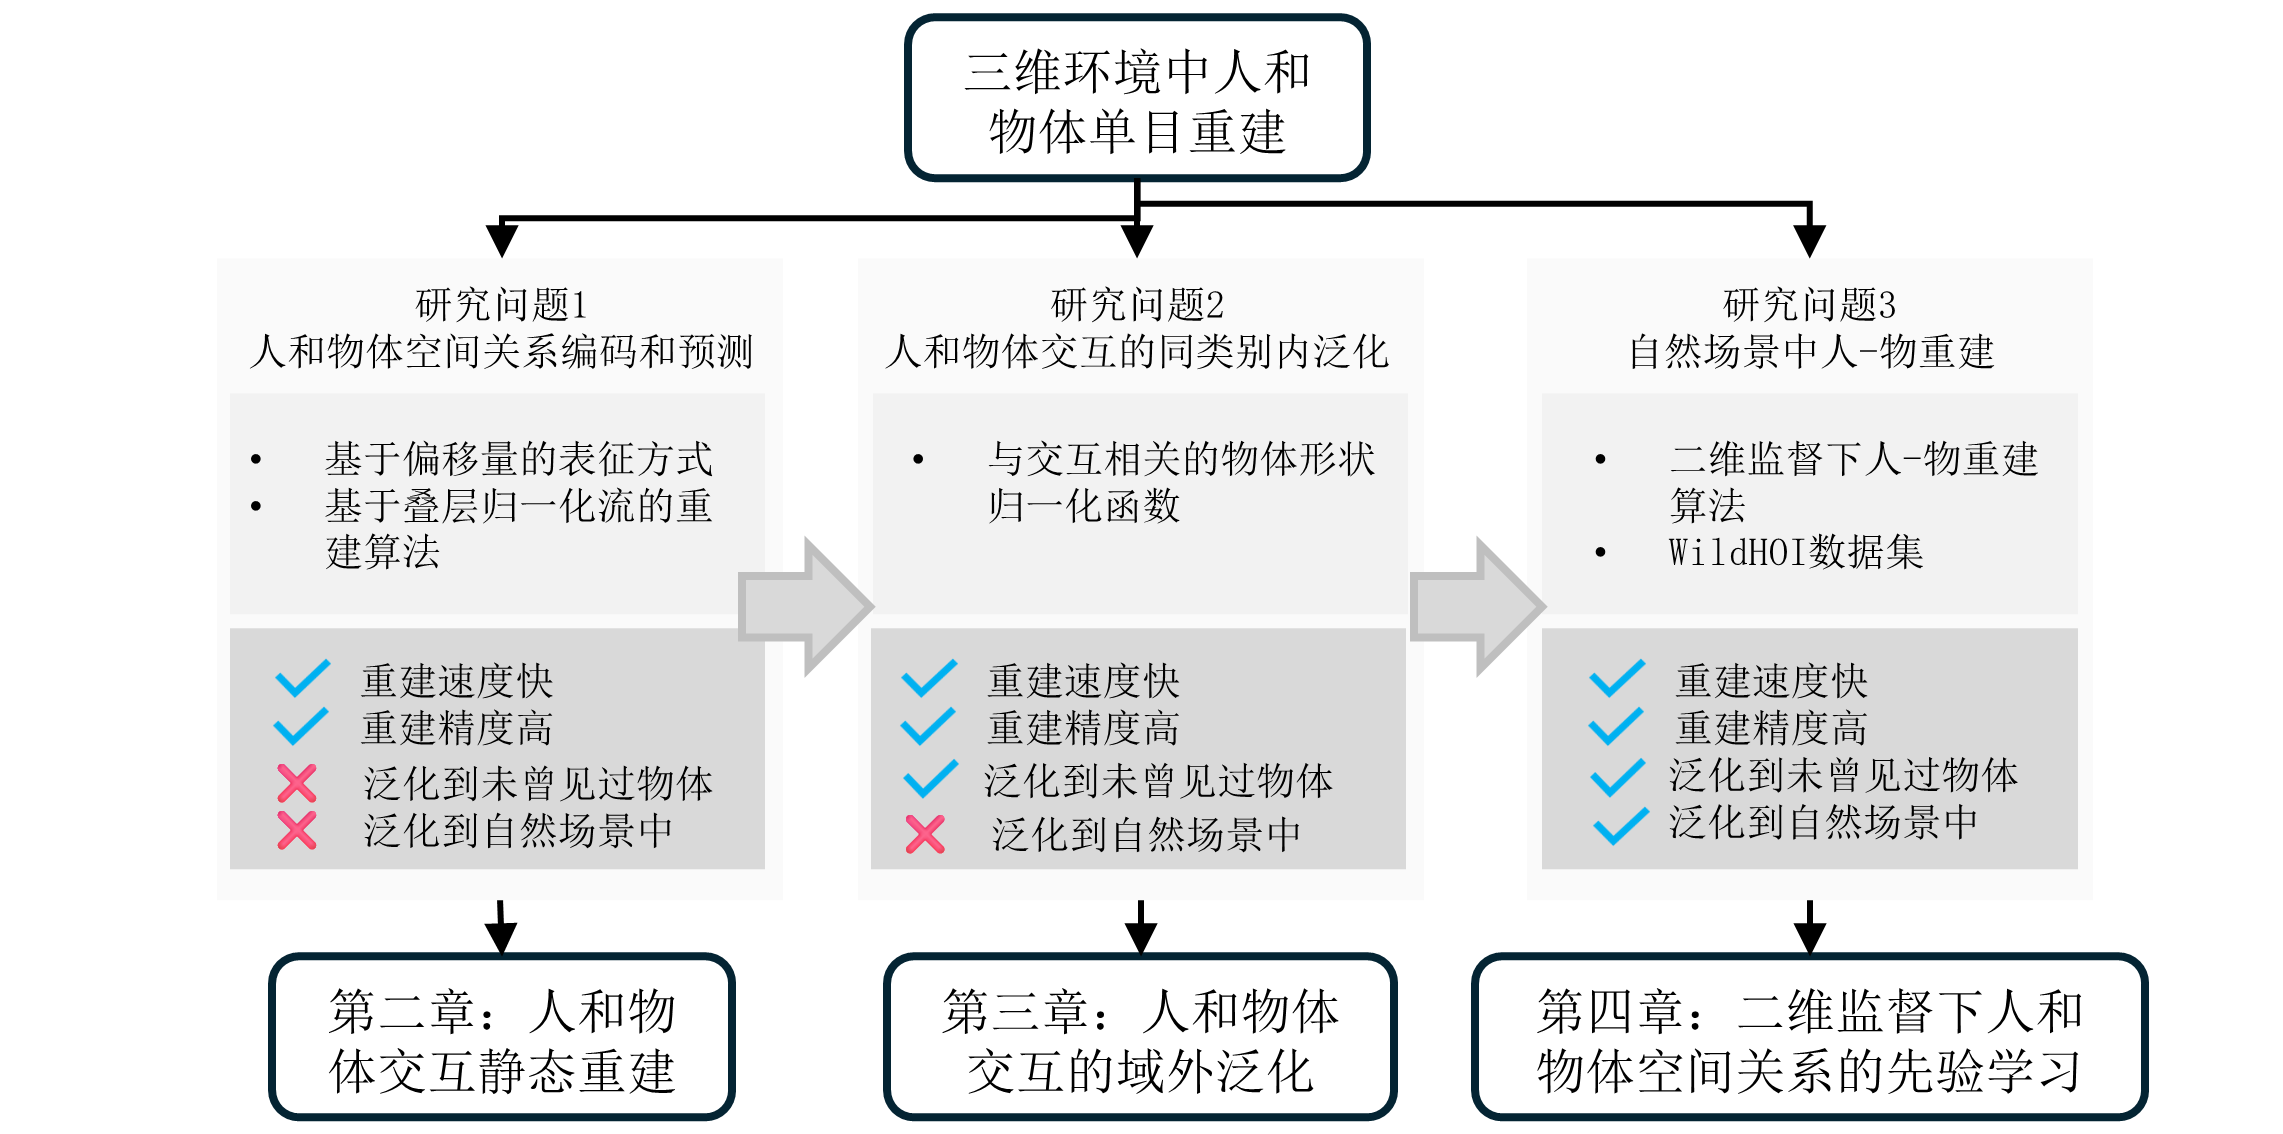
\includegraphics{Img/paper_structure}
	\bicaption{本文章节组织结构。}{The organizational structure of this thesis.}
	\label{fig:structure}
\end{figure}

\section{本文组织结构}

本文的主要研究内容是从单张图片中联合重建出人和物体,针对人-物空间关系建模、人-物空间关系域外泛化和二维监督下的三维人-物关系先验学习三方面提出了一系列创新型算法。本文包含五个章节,如图\ref{fig:structure}所示,其具体组织如下:

\textbf{第一章,绪论。} 主要介绍人和物体交互单目重建的研究背景,指出人-物交互在各个领域的重要性和应用前景,并探讨了现存方法存在重建速度低、泛化能力差和严重依赖于三维标签的缺点,并引出本文的主要工作内容和创新点,最后对本文各个章节做出总述。

\textbf{第二章,人和物体交互静态重建。} 介绍基于偏移量的人和物体空间关系的编码方法,描述了叠层归一化的重建算法,展示了算法在BEHAVE上的性能对比。

\textbf{第三章,人和物体交互的域外泛化。} 给出物体形状归一化映射函数结构和类别级的重建算法,展示了在CHAIRS数据集上的实验结果。

\textbf{第四章,二维监督下人和物体空间关系的先验学习。} 提出从二维图片提取三维空间关系先验的一种二维信息监督的方法,描述了构建自然场景中数据集的流程,在BEHAVE数据集和自然场景数据集中和之前先进方法进行了对比分析。


\textbf{第五章,总结与展望。} 总结了本文的主要研究内容,并展望了未来的研究方向。


% \textbf{第一章,绪论。} 在第一章中,主要介绍人和物体交互单目重建的研究背景,指出人-物交互在各个领域的重要性和应用前景,并探讨了现存方法存在重建速度低、泛化能力差和严重依赖于三维标签的缺点,并引出本文的主要工作内容和创新点,最后对本文各个章节做出总述。

% \textbf{第二章,人和物体交互静态重建。} 在第二章中,首先介绍基于偏移量的人和物体空间关系的编码方法,并描述了基于该偏移量表示的叠层归一化模型结构,以及基于归一化流的单目重建算法,在实验中,重点在BEHAVE数据集和InterCap数据集和先前方法进行了对比,并进行大量的消融实验和对比实验以表明该算法的有效性。

% \textbf{第三章,人和物体交互的域外泛化。} 在第三章中,提出了前置章节存在的问题和局限性并进一步引出本章的算法,为提高算法对新物体的泛化能力,给出物体形状归一化映射函数结构和类别级的重建算法,最后展示了在CHAIRS数据集上的实验结果,通过和基于RT的方法相比说明本章算法能够对训练集中未曾见过物体的泛化能力。

% \textbf{第四章,二维监督下人和物体空间关系的先验学习。} 在第四章中,针对之前章节严重依赖于三维标注数据而不能泛化到自然场景中的缺陷,提出了从二维图片提取三维空间关系先验的一种二维信息监督的方法,描述了构建自然场景中数据集的流程,在BEHAVE数据集和自然场景数据集中和之前先进方法进行了对比分析。

% \textbf{第五章,总结与展望。} 在第五章中,总结了本文的主要研究内容,并在探索人-物空间关系表征、使用先验来提高泛化能力和模型到自然场景中的迁移等方面展望了未来的研究方向。